\documentclass[12pt,reqno]{article}
\usepackage{amsthm, amsmath, amsfonts, amssymb, amscd, mathtools, youngtab, euscript, mathrsfs, verbatim, enumerate, multicol, multirow, bbding, color, babel, esint, geometry, tikz, tikz-cd, tikz-3dplot, array, enumitem, hyperref, thm-restate, thmtools, datetime, graphicx, tensor, braket, slashed, standalone, pgfplots, ytableau, subfigure, wrapfig, dsfont, setspace, wasysym, pifont, float, rotating, adjustbox, pict2e,array}
\usepackage{amsmath}
\usepackage[utf8]{inputenc}
\usetikzlibrary{arrows, positioning, decorations.pathmorphing, decorations.pathreplacing, decorations.markings, matrix, patterns}
\tikzset{big arrow/.style={
    decoration={markings,mark=at position 1 with {\arrow[scale=1.5,#1]{>}}},
    postaction={decorate},
    shorten >=0.4pt},
  big arrow/.default=black}

\begin{document}

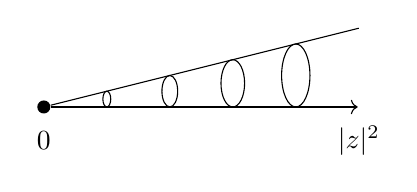
\begin{tikzpicture}
\node[circle,thick,scale=0.5,fill=black,label={[label distance=1mm]south:$0$}] (A1) at (0,0) {};
\node[draw=none,opacity=0,thick,scale=0.1,fill=black,label={[label distance=1mm]south:$|z|^2$}] (A2) at (4,0) {};
\draw[->] (A1)--(A2);
\draw (A1)--(4,1);
\draw (0.8,0.1) ellipse (0.05cm and 0.1cm);
\draw (1.6,0.2) ellipse (0.1cm and 0.2cm);
\draw (2.4,0.3) ellipse (0.15cm and 0.3cm);
\draw (3.2,0.4) ellipse (0.18cm and 0.4cm);
\end{tikzpicture}

\end{document}